
\documentclass[a4paper,11pt]{article}
\usepackage[a4paper, margin=8em]{geometry}

% usa i pacchetti per la scrittura in italiano
\usepackage[french,italian]{babel}
\usepackage[T1]{fontenc}
\usepackage[utf8]{inputenc}
\frenchspacing 

% usa i pacchetti per la formattazione matematica
\usepackage{amsmath, amssymb, amsthm, amsfonts}

% usa altri pacchetti
\usepackage{gensymb}
\usepackage{hyperref}
\usepackage{standalone}

% imposta il titolo
\title{Appunti Fondamenti di Automatica}
\author{Luca Seggiani}
\date{2025}

% disegni
\usepackage{pgfplots}
\pgfplotsset{width=10cm,compat=1.9}

% imposta lo stile
% usa helvetica
\usepackage[scaled]{helvet}
% usa palatino
\usepackage{palatino}
% usa un font monospazio guardabile
\usepackage{lmodern}

% tikz in sans
\tikzset{every picture/.style={/utils/exec={\sffamily}}}

\renewcommand{\rmdefault}{ppl}
\renewcommand{\sfdefault}{phv}
\renewcommand{\ttdefault}{lmtt}

% circuiti
\usepackage{circuitikz}
\usetikzlibrary{babel}

% disponi il titolo
\makeatletter
\renewcommand{\maketitle} {
	\begin{center} 
		\begin{minipage}[t]{.8\textwidth}
			\textsf{\huge\bfseries \@title} 
		\end{minipage}%
		\begin{minipage}[t]{.2\textwidth}
			\raggedleft \vspace{-1.65em}
			\textsf{\small \@author} \vfill
			\textsf{\small \@date}
		\end{minipage}
		\par
	\end{center}

	\thispagestyle{empty}
	\pagestyle{fancy}
}
\makeatother

% disponi teoremi
\usepackage{tcolorbox}
\newtcolorbox[auto counter, number within=section]{theorem}[2][]{%
	colback=blue!10, 
	colframe=blue!40!black, 
	sharp corners=northwest,
	fonttitle=\sffamily\bfseries, 
	title=Teorema~\thetcbcounter: #2, 
	#1
}

% disponi definizioni
\newtcolorbox[auto counter, number within=section]{definition}[2][]{%
	colback=red!10,
	colframe=red!40!black,
	sharp corners=northwest,
	fonttitle=\sffamily\bfseries,
	title=Definizione~\thetcbcounter: #2,
	#1
}

% disponi problemi
\newtcolorbox[auto counter, number within=section]{problem}[2][]{%
	colback=green!10,
	colframe=green!40!black,
	sharp corners=northwest,
	fonttitle=\sffamily\bfseries,
	title=Problema~\thetcbcounter: #2,
	#1
}

% disponi codice
\usepackage{listings}
\usepackage[table]{xcolor}

\lstdefinestyle{codestyle}{
		backgroundcolor=\color{black!5}, 
		commentstyle=\color{codegreen},
		keywordstyle=\bfseries\color{magenta},
		numberstyle=\sffamily\tiny\color{black!60},
		stringstyle=\color{green!50!black},
		basicstyle=\ttfamily\footnotesize,
		breakatwhitespace=false,         
		breaklines=true,                 
		captionpos=b,                    
		keepspaces=true,                 
		numbers=left,                    
		numbersep=5pt,                  
		showspaces=false,                
		showstringspaces=false,
		showtabs=false,                  
		tabsize=2
}

\lstdefinestyle{shellstyle}{
		backgroundcolor=\color{black!5}, 
		basicstyle=\ttfamily\footnotesize\color{black}, 
		commentstyle=\color{black}, 
		keywordstyle=\color{black},
		numberstyle=\color{black!5},
		stringstyle=\color{black}, 
		showspaces=false,
		showstringspaces=false, 
		showtabs=false, 
		tabsize=2, 
		numbers=none, 
		breaklines=true
}

\lstdefinelanguage{javascript}{
	keywords={typeof, new, true, false, catch, function, return, null, catch, switch, var, if, in, while, do, else, case, break},
	keywordstyle=\color{blue}\bfseries,
	ndkeywords={class, export, boolean, throw, implements, import, this},
	ndkeywordstyle=\color{darkgray}\bfseries,
	identifierstyle=\color{black},
	sensitive=false,
	comment=[l]{//},
	morecomment=[s]{/*}{*/},
	commentstyle=\color{purple}\ttfamily,
	stringstyle=\color{red}\ttfamily,
	morestring=[b]',
	morestring=[b]"
}

% disponi sezioni
\usepackage{titlesec}

\titleformat{\section}
	{\sffamily\Large\bfseries} 
	{\thesection}{1em}{} 
\titleformat{\subsection}
	{\sffamily\large\bfseries}   
	{\thesubsection}{1em}{} 
\titleformat{\subsubsection}
	{\sffamily\normalsize\bfseries} 
	{\thesubsubsection}{1em}{}

% disponi alberi
\usepackage{forest}

\forestset{
	rectstyle/.style={
		for tree={rectangle,draw,font=\large\sffamily}
	},
	roundstyle/.style={
		for tree={circle,draw,font=\large}
	}
}

% disponi algoritmi
\usepackage{algorithm}
\usepackage{algorithmic}
\makeatletter
\renewcommand{\ALG@name}{Algoritmo}
\makeatother

% disponi numeri di pagina
\usepackage{fancyhdr}
\fancyhf{} 
\fancyfoot[L]{\sffamily{\thepage}}

\makeatletter
\fancyhead[L]{\raisebox{1ex}[0pt][0pt]{\sffamily{\@title \ \@date}}} 
\fancyhead[R]{\raisebox{1ex}[0pt][0pt]{\sffamily{\@author}}}
\makeatother

\begin{document}

% sezione (data)
\section{Lezione del 01-04-25}

% stili pagina
\thispagestyle{empty}
\pagestyle{fancy}

% testo
\subsubsection{Derivazione alternativa della funzione sottosmorzata}
Avevamo ricavato l'espressione nella 13.0.2:
$$
y(t) = \frac{b_0}{a_0} \left( 1 - e^{\alpha t} \cos(\beta t) + \frac{\alpha}{\beta} e^{\alpha t} e^{\alpha t} \sin(\beta t) \right) \cdot H(t)
$$
per la risposta al gradino edi sistemi del second'ordine sottosmorzati.
Notiamo l'esistenza della forma (equivalente):
$$
y(t) = G(0) \cdot \left( 1 - e^{-\xi \omega t} \cos\left(\omega \sqrt{1 - \xi ^2} \cdot t \right) - \frac{\xi}{\sqrt{1 - \xi^2}} e^{-\xi \omega t} \sin\left( \omega \sqrt{1 - \xi^2} \cdot t \right) \right) \cdot H(t)
$$
che evidenzia la dipendenza dal guadagno $G(0)$, e dai valori di pulsazione naturale $\omega$ e smorzamento $\xi$.
Vediamo quindi come si può svolgere una derivazione (con 2 procedimenti leggermente diversi), formale, attraverso Laplace (visto che precedentemente siamo andati avanti per stime).

\begin{enumerate}
	\item Partiamo dalla forma di Evans della funzione di trasferimento della 13.0.2:
		$$
		G(s) = G(0) \cdot \frac{\omega^2}{s^2 + 2 \omega \xi \cdot s + \omega^2}
		$$
		Da cui la risposta al gradino:
		$$
		Y(s) = G(s) \cdot U(s) = G(0) \cdot \frac{\omega^2}{\left( s^2 + 2 \omega \xi \cdot s + \omega^2 \right) s}
		$$
		Dal denominatore si ha il polo semplice $p_0 = 0$ e i poli complessi coniugati $p_{1,2}$:
		$$
		p_{1,2} = - \frac{ - 2 \xi \omega \pm \sqrt{4 \xi^2 \omega^2 - 4 \omega^2} }{2} = - \frac{ - 2 \xi \omega \pm 2 \omega \sqrt{\xi^2 - 1} }{2} = \xi \omega \mp \omega \sqrt{1 - \xi^2}
		$$
		che equivale a quanto avevamo già trovato:
		$$
		p_{1, 2} = -(\alpha \pm i \beta), \quad \alpha = -\xi \omega, \quad \beta = \omega \sqrt{1 - \xi^2}
		$$
		Possiamo quindi portare la funzione nel dominio di Laplace nella forma a fratti semplici:
		$$
		Y(s) = G(0) \cdot \left( \frac{A}{s} + \frac{B}{s + p_1} + \frac{B^*}{s + p_2} \right)
		$$
		avevamo già calcolato $A$ attraverso il teorema dei residui:
		$$
		A = \lim_{s \rightarrow 0} \frac{ \omega^2 }{ s^2 + 2 \omega \xi \cdot s + \omega^2 } = 1 
		$$
		Per $B$ e $B^*$, svolgiamo la somma:
		$$
		Y(s) = G(0) \cdot \left( \frac{1}{s} + \frac{B}{s + p_1} + \frac{B}{s + p_2} \right) 
		$$
		$$
		= G(0) \cdot \frac{ (s + p_1)(s + p_2) + Bs(s + p_2) + B^*s(s + p_1) }{(s + p_1)(s + p_2)s}
		$$
		$$
		= G(0) \cdot \frac{ s^2 + p_2 s + p_1 s + p_1 p_2 + Bs^2 + B p_2 s + B^* s^2 + B^* p_1 s }{(s + p_1)(s + p_2)s}
		$$
	vogliamo eguagliare il numeratore a $\omega^2$, in modo da rispettare la forma di Evans.
	Abbiamo quindi che l'unico termine costante è $p_1 p_2$, che vale:
	$$
	p_1 p_2 = -(\alpha + i \beta) \cdot -(\alpha - i \beta) = \alpha^2 - \beta^2 = \xi^2 \omega^2 + \omega^2 (1 - \xi^2) = \omega^2
	$$
	Quindi tutto quello che ci serve è che sia soddisfatto il sistema:
	\[
		\begin{cases}
			1 + B + B^* = 0 \\ 
			p_2 + p_1 + B p_2 + B^* p_1 = 0
		\end{cases}
	\]
	Dalla prima equazione ricaviamo:
	$$
	B^* = - (1 + B) \implies p_2 + p_1 + B p_2 - (1 + B)p_1 = p_2 + B p_2 - B p_1  = 0
	$$
	da cui:
	$$
	B = - \frac{p_2}{p_2 - p_1} = \frac{\alpha - i \beta}{- \alpha + i \beta + \alpha + i \beta} = \frac{\alpha - i \beta}{ i 2 \beta} = - \frac{i\alpha + \beta}{2 \beta} = -\frac{1}{2} \left( 1 + i\frac{\alpha}{\beta} \right) 
	$$
	che sostituendo in $Y(s)$ dà:
	$$
	Y(s) = G(0) \cdot \left( \frac{1}{s} - \frac{ \frac{1}{2} \left( 1 + i \frac{\alpha}{\beta} \right) }{s + p_1} - \frac{ \frac{1}{2} \left( 1 - i \frac{\alpha}{\beta} \right) }{s + p_2} \right)
	$$
	Procediamo quindi con l'antitrasformazione:
	$$
	\mathcal{L}^{-1} \left\{ Y(s) \right\} = G(0) \cdot \left( 1 - \frac{1}{2} \left( 1 + i \frac{\alpha}{\beta} \right) e^{\alpha t} e^{i \beta t} - \frac{1}{2} \left( 1 - i \frac{\alpha}{\beta} \right) e^{\alpha t} e^{-i \beta t} \right) \cdot H(t)
	$$
	$$
	= G(0) \cdot \left( 1 - \frac{1}{2} \left( 1 + i \frac{\alpha}{\beta} \right) e^{\alpha t} \left( \cos(\beta t) + \sin(\beta t) \right) \right.
	$$
	$$
	\hspace{3.4cm} \left. - \frac{1}{2} \left( 1 - i \frac{\alpha}{\beta} \right) e^{\alpha t} \left( \cos(\beta t) - \sin(\beta t) \right) \right) \cdot H(t)
	$$
	$$
	= G(0) \cdot \left( 1 + e^{\alpha t} \cdot \left( - \frac{1}{2} \cos(\beta t) - i \frac{1}{2} \sin(\beta t) - i \frac{\alpha}{\beta} \cos(\beta t) + \frac{\alpha}{\beta} \sin(\beta t) \right. \right.
	$$
	$$
	\hspace{4.5cm}  \left. \left. - \frac{1}{2} \cos(\beta t) + i \frac{1}{2} \sin(\beta t) + i \frac{\alpha}{\beta} \cos(\beta t) + \frac{\alpha}{\beta} \sin(\beta t) \right) \right) \cdot H(t)
	$$
	$$
	= G(0) \cdot \left( 1 - e^{\alpha t} \cos(\beta t) + \frac{\alpha}{\beta} \sin(\beta t) \right) \cdot H(t)
	$$ \qed

\item Prendiamo come forma a fratti semplici:
	$$
	Y(s) = G(0) \cdot \left( \frac{A}{s} + \frac{Bs + C}{s^2 + 2\omega \xi \cdot s + \omega^2} \right) = G(0) \cdot \left( \frac{1}{s} + \frac{Bs + C}{s^2 + 2\omega \xi \cdot s + \omega^2} \right) 
	$$
	visto che $A$ è sempre lo stesso residuo di prima.
	Svolgendo le moltiplicazioni si ha:
	$$
	 = G(0) \cdot \left( \frac{s^2 + 2 \omega \xi \cdot s + \omega^2 + Bs^2 + Cs}{s (s^2 + 2 \omega \xi s + \omega^2)} \right)
	$$
	di cui il sistema:
	\[
		\begin{cases}
			1 + B = 0 \\ 
			2 \omega \xi + C
		\end{cases} \implies
		\begin{cases}
			B = -1 \\ 
			C = - 2 \omega \xi	
		\end{cases}
	\]
	Sostituendo si ha quindi:
	$$
	Y(s) = G(0) \cdot \left( \frac{1}{s} - \frac{s + 2 \omega \xi}{s^2 + 2 \omega \xi \cdot s + \omega^2} \right)
	$$
	Prendiamo il termine ad destra singolarmente, e riscriviamo come:
	$$
	\frac{s + 2 \omega \xi}{s^2 + 2 \omega \xi \cdot s + \omega^2} = \frac{(s + \omega \xi) + \omega \xi}{(s + \omega \xi)^2 - \omega \xi^2 + \omega^2} = \frac{(s+ \omega \xi) + \omega \xi}{(s + \omega \xi)^2 + \omega^2 (1 - \xi^2)} 
	$$
	da cui la forma più adatta alla trasformazione:
	$$
	= \frac{(s+ \omega \xi) + \omega \xi \sqrt{ \frac{1 - \xi^2}{1 - \xi^2} }}{(s + \omega \xi)^2 + \omega^2 (1 - \xi^2)} = \frac{s + \omega \xi}{(s + \omega \xi)^2 + \omega^2 (1 - \xi^2)} + \frac{ \omega \xi \sqrt{ \frac{1 - \xi^2}{1 - \xi^2} } }{(s + \omega \xi)^2 + \omega^2 (1 - \xi^2)}
	$$
	$$
	= \frac{s + \omega \xi}{(s + \omega \xi)^2 + \omega^2 (1 - \xi^2)} + \frac{\xi}{\sqrt{1 - \xi^2}} \frac{ \omega \sqrt{ 1 - \xi^2 } }{(s + \omega \xi)^2 + \omega^2 (1 - \xi^2)}
	$$
	Basterà quindi riconoscere che, preso $\omega_d = \omega \sqrt{1 - \xi^2}$ e $a = -\omega \xi$, si che i due termini sono immediatamente trasformabili secondo Laplace come oscillanti scostati in tempo, quindi attraverso:
	$$
	\mathcal{L}^{-1} \left\{ \cos(\omega t) \right\} = \frac{s}{s^2 + \omega^2}, \quad \mathcal{L}^{-1} \left\{ \sin(\omega t) \right\} = \frac{\omega}{s^2 + \omega^2}
	$$
	per i termini oscillanti e:
	$$
	\mathcal{L}^{-1} \left\{ F(s - a) \right\} = e^{at} f(t)
	$$
	per lo scostamento temporale, si ha:
	$$
	\implies e^{-\omega \xi t} \cos\left(\omega \sqrt{ 1- \xi^2} \cdot t\right) + \frac{\xi}{\sqrt{1 - \xi^2}} e^{-\omega \xi t} \sin\left(\omega \sqrt{1 - \xi^2} \cdot t\right)
	$$
	che risulta nella $y(t)$:
	$$
y(t) = G(0) \cdot \left( 1 - e^{-\xi \omega t} \cos\left(\omega \sqrt{1 - \xi ^2} \cdot t \right) - \frac{\xi}{\sqrt{1 - \xi^2}} e^{-\xi \omega t} \sin\left( \omega \sqrt{1 - \xi^2} \cdot t \right) \right) \cdot H(t)
	$$ \qed
\end{enumerate}

Il lato destro dell'espressione trovata si può chiaramente riscrivere nella forma più concisa $ke^{-\sigma t} \sin(\omega t + \alpha)$. 
Usiamo allora le formule di traduzione in forma sinusoidale, di cui una dimostrazione nel caso cosinusoidale si trova a \url{https://github.com/seggiani-luca/appunti-fis/blob/main/master/master.pdf}:
\[
	c_1 \sin{\omega t} + c_2 \cos{\omega t}
	\Leftrightarrow
	k \sin(\omega t + \alpha)
\]
con:
\[
	\begin{cases}
		k 	= \sqrt{c_1^2 + c_2^2} \\ 
		\alpha = \tan^{-1}(\frac{c1}{c2})
	\end{cases}
\]

che darà quindi:
$$
y(t) = G(0) \cdot \left( 1 - e^{-\xi \omega t} \sqrt{1 + \frac{\xi^2}{1 + \xi^2}} \sin\left( \omega \sqrt{1 - \xi^2} \cdot t + \tan^{-1} \left( \frac{\sqrt{1 - \xi^2}}{\xi} \right) \right) \right) 
$$

\noindent
\begin{minipage}{\textwidth}
\subsection{Dettaglio sulla risposta dei sistemi sottosmorzati}
Vediamo in particolare alcune grandezze di interesse nel caso di sistemi di secondo grado sottosmorzati:

\par\bigskip

\begin{center}
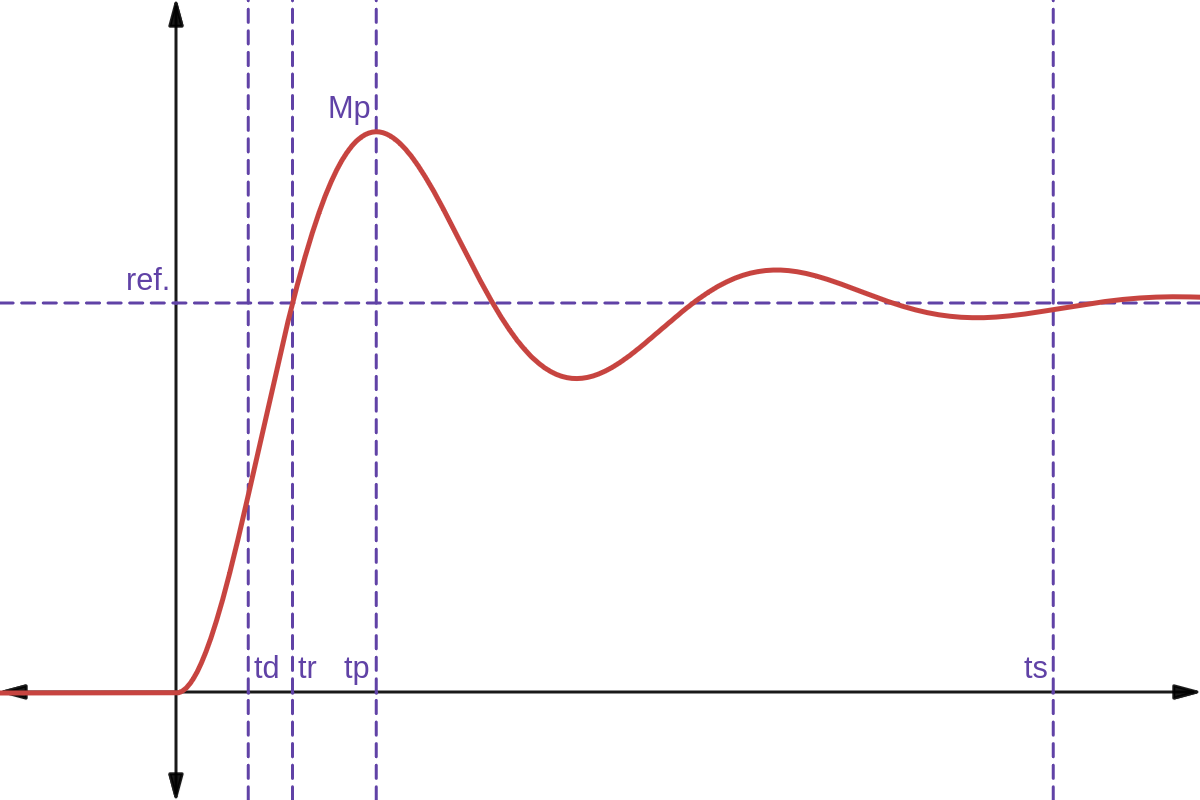
\includegraphics[scale=0.29]{../figures/damped_oscillator.png}
\end{center}
\end{minipage}

\par\bigskip

Abbiamo che una caratteristica del loro comportamento è la \textbf{sovraelongazione} al di sopra del valore bersaglio.
Chiamiamo quindi $M_p$ la \textit{massima sovraelongazione} sopra il livello di riferimento, e $t_p$ l'istante temporale in cui questa viene raggiunta.
Avremo poi il tempo $t_r$ \textit{di salita}, il momento in cui viene toccato per la prima volta il valore bersaglio, e il tempo $t_d$ \textit{di ritardo}, che viene impiegato a raggiungere il 50\% del valore bersaglio.
Infine, per valutare il comportamento oscillante dopo il transiente iniziale, consideriamo il tempo $t_s$ \textit{di assestamento}, oltre il quale il segnale resta in una certa (piccola) percentuale del valore bersaglio.

Notiamo che possiamo considerare gli stessi parametri considerati sui sistemi sottosmorzati anche per sistemi criticamente smorzati o sovrasmorzati: infatti, se non per il tempo e per il punto di sovraelengazione, questi avranno valori ben definiti per qualsiasi sistema del second'ordine.

Tornando al dettaglio dei sistemi sottosmorzati, possiamo trovare le seguenti formule:
\begin{itemize}
	\item \textbf{Sovraelongazione:} 
		\begin{theorem}{Sovraelongazione di sottosmorzate}
			Si ha il picco di una sottosmorzata in:
		$$
			S\% \ (M_p) \ = 100 e^{- \frac{\xi \pi}{\sqrt{1 - \xi^2}}}
		$$
		raggiunto all'istante:
		$$
			t_p = \frac{\pi}{\omega \sqrt{1 - \xi^2}}
		$$

		\end{theorem}
		Queste derivano dal punto di massimo della funzione $y(t)$:
		$$
		y(t) = G(0) \cdot \left( 1 - e^{-\xi \omega t} \cos\left(\omega \sqrt{1 - \xi ^2} \cdot t \right) - \frac{\xi}{\sqrt{1 - \xi^2}} e^{-\xi \omega t} \sin\left( \omega \sqrt{1 - \xi^2} \cdot t \right) \right) \cdot H(t)
		$$
		da cui:
		$$
		D \left[ y(t) \right] \propto \xi \omega e^{-\xi \omega \cdot t} \sin\left( \omega \sqrt{1 - \xi^2} t + \phi \right) - e^{-\xi \omega t} \omega \sqrt{1 - \xi^2} \cos\left( \omega \sqrt{1 - \xi^2} \cdot t + \phi \right)
		$$
		$$
		\propto \xi \sin\left( \omega \sqrt{1 - \xi^2} \cdot t + \phi \right) - \sqrt{1 - \xi^2} \cos\left( \omega \sqrt{1 - \xi^2 \cdot t + \phi} \right)
		$$
		che si porta alla forma sinusoidale con:
		\[
			\begin{cases}
				k = \sqrt{ \xi^2 + 1 - \xi^2 } = 1 \\
				\phi' = \tan^{-1} \left( -\frac{\xi}{\sqrt{1 - \xi^2}} \right)
			\end{cases}
		\]
		da cui:
		$$
		\propto \sin\left( \omega \sqrt{1 - \xi^2} \cdot t + \phi + \phi' \right) = \sin\left( \omega \sqrt{1 - \xi^2} \cdot t \right)
		$$
		che ha il primo zero dopo $t = 0$ in $t_p = \frac{\pi}{\omega \sqrt{1 - \xi^2}}$ (quando il seno ha argomento $\pi$). \qed
		
		Prendendo il valore di $y(t)$ in $t_p$ si ha che resta solo il coseno, cioè:
		$$
		y(t_p) = G(0) \cdot (1 + e^{\xi \omega t_p})
		$$
		da cui $e^{\xi \omega t_p}$ rappresenta la frazione di surplus al punto di massimo sovraelongamento, che moltiplichiamo per 100 per portare in percentuale. \qed
	\item \textbf{Periodo di oscillazione:}
		\begin{theorem}{Periodo di oscillazione di sottosmorzate}
		Una sottosmorzata ha periodo di oscillazione:
			$$
			T_o = \frac{2\pi}{\omega \sqrt{1 - \xi^2}}
		$$
		e frequenza:
		$$
			f_o = \frac{\omega \sqrt{1 - \xi^2}}{2\pi} 
		$$
		\end{theorem}
		Queste derivano dalla componente complessa $\beta$ dei poli, o direttamente dalla pulsazione effettiva:
		$$
		\omega_d = \omega \sqrt{1 - \xi^2}
		$$
	\item \textbf{Tempo di assestamento:} consideriamo questo come:
		$$
		t_s \approx -\frac{1}{\xi \omega} \ln(0.05)
		$$
		trascurando la componente oscillante e prendendo il punto dove il solo esponenziale raggiunge il 5\% del suo valore massimo (in decadimento):
		$$
		e^{-\omega \xi t_s} = 0.05, \quad -\omega \xi t = \ln (0.05) \implies t_s \approx -\frac{1}{\xi \omega} \ln(0.05)
		$$
	\item \textbf{Tempo di salita:} consideriamo infine questo, con molta approssimazione, come:
		$$
		t_r \approx \frac{1.8}{\omega}
		$$
\end{itemize}

\subsubsection{Comportamento al variare dello smorzamento}
\noindent
\begin{minipage}{\textwidth}
Concludiamo il discorso sui sistemi sottosmorzati considerando il comportamento generale dei sistemi di questo tipo al variare del valore di smorzamento $\xi = \frac{a_1}{2 \sqrt{a_0 a_2}}$:

\par\bigskip

\begin{center}
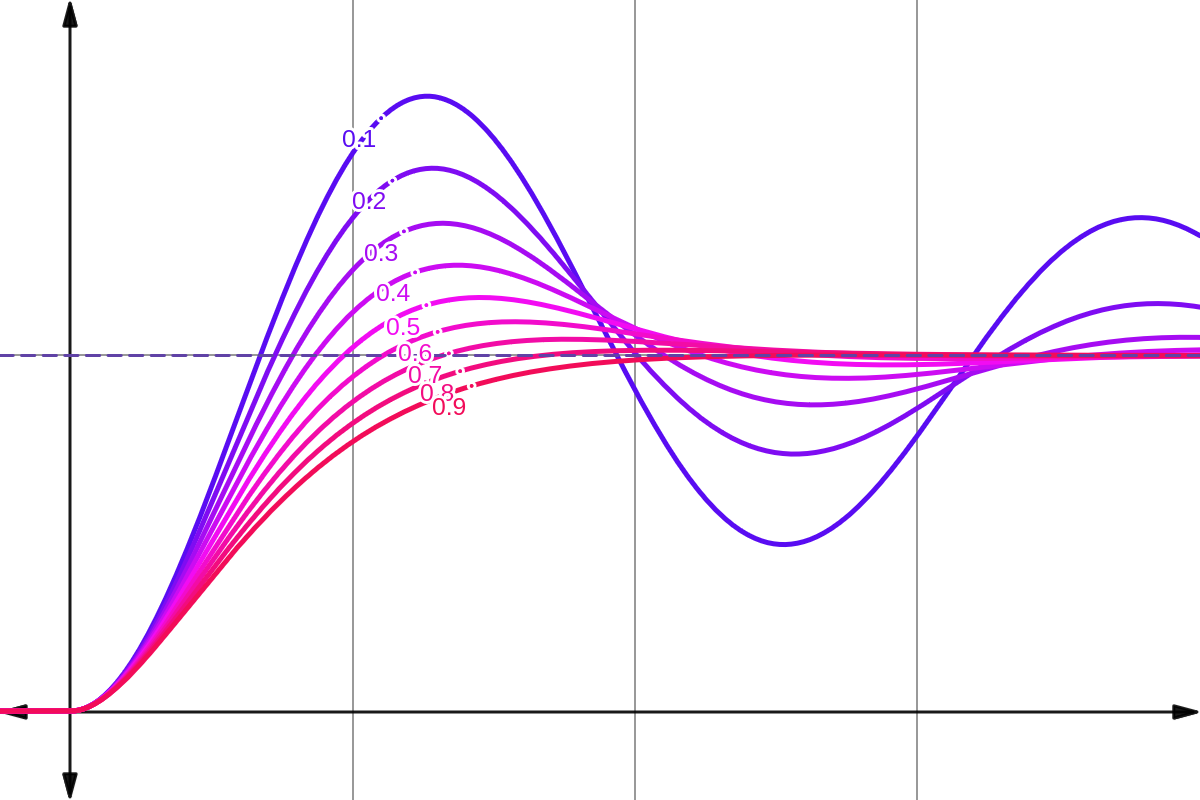
\includegraphics[scale=0.29]{../figures/damping_values.png}
\end{center}
\end{minipage}

\par\bigskip

Da dove notiamo che a valori di smorzamento maggiori si ha minore sovraelongamento, ma anche maggiore tempo di salita.

\subsection{Stabilità nel modello a funzione di trasferimento}
Abbiamo lavorato finora col modello a funzione di trasferimento, definita come:
$$
G(s) = \frac{\sum_{i = 0}^m b_i s^i}{\sum_{i = 0}^n a_i s^i} = \frac{ b_m (s - z_1) (s - z_2) ... (s - z_m) }{ a_n (s - p_1) (s - p_2) ... (s - p_n) }
$$
con $z_i$ gli $m$ \textit{zeri}, $p_i$ gli $n$ \textit{poli}, e $n > m$.

Di questa avevamo individuato le due forme:
\begin{itemize}
	\item \textbf{Forma di Evans:} evidenzia poli e zeri:
		$$
G(s) = \frac{\sum_{i = 0}^m b_i s^i}{\sum_{i = 0}^n a_i s^i} = \frac{ b_m (s - z_1) (s - z_2) ... (s - z_m) }{ a_n (s - p_1) (s - p_2) ... (s - p_n) }
		$$
	\item \textbf{Forma di Bode:} evidenzia le costanti tempo: 
		$$
G(s) = K \frac{ (\tau_a s + 1) (\tau_b s + 1) ... (\tau_i s + 1) }{ (\tau_1 s + 1) (\tau_2 s + 1) ... (\tau_n s + 1) }
		$$
\end{itemize}

Definiamo quindi formalmente \textbf{poli}:
\begin{definition}{Polo}
	Un polo $a_i$ di una funzione di trasferimento $G(s)$ è un valore di $s$ per cui $G(s)$ tende ad infinito:
	$$
	F(s) = \frac{g(s)}{\prod_{i = 1}^x (s - a_i)^n_i}
	$$
	con $n_i$ ordine del polo.
\end{definition}
e \textbf{zeri}:
\begin{definition}{Zeri}
	Uno zero $a_i$ di una funzione di trasferimento $G(s)$ è un valore di $s$ per cui $G(s)$ tende a zero: 
	$$
	F(s) = \frac{\prod_{i = 1}^x (s - a_i)^m_i}{g(s)}
	$$
	con $m_i$ ordine dello zero.
\end{definition}

Quello che ci interesserà nella valutazione della \textbf{stabilità} dei sistemi sarà la posizione dei poli nel piano complesso.
In particolare, come avevamo detto per i modi nel modello a variabili di stato, poli a componente \textit{reale negativa} danno \textbf{stabilità asintotica}, poli a componente \textit{reale nulla} danno \textbf{stabilità marginale}, e poli a componente \textit{reale positiva} dano \textbf{instabilità}.
Inoltre la componente \textit{complessa} dà informazioni sull'oscillazione del sistema, con \textbf{oscillazioni smorzate} a componente \textit{complessa e reale non nulle}, e \textbf{oscillazioni continue} a componente \textit{reale nulla}.

Gli zeri, invece, non hanno effetto sulla stabilità.
Gli zeri a parte reale positiva hanno invece l'effetto di \textit{invertire} la risposta al gradino, almeno sul breve termine.

\subsubsection{Conversione da spazio di stato a funzione di trasferimento}
Dovrebbe ormai essere chiaro che lo spazio di stato e la funzione di trasferimento rappresentano due modi di modelizzare lo stesso tipo di fenomeni.
Vediamo quindi come passare dall'uno all'altro.

Partiamo dal modello a variabili di stato:
\[
	\begin{cases}
		x' = Ax + Bu \\
		y = Cx + Du
	\end{cases}
\]

Assumendo condizioni iniziali nulle, si ha:
\[
	\begin{cases}
		s X(s) = A X(s) + B U(s)  \\ 
		Y(s) = C X(s) + D U(s) 
	\end{cases} \implies
	\begin{cases}
		X(s) = (sI - A)^{-1} B U(s) \\
		Y(s) = \left( C(sI - A)^{-1} B + D \right) U(s)
	\end{cases}
\]
notando che $X, U$ sono vettori e $A, B$ matrici.

Si trova quindi la funzione di trasferimento:
$$
G(s) = \frac{Y(s)}{U(s)} = C(sI - A)^{-1} B + D
$$

\subsubsection{Forme canoniche di controllo}
Esistono un numero infinito di possibili modelli in spazio di stato che forniscono la stessa dinamica ingresso/uscita.

Aiuta avere alcune strutture standardizzate dei modelli in spazio di stato: queste sono le cosiddette forme canoniche.
Data la funzione di trasferimento di un sistema, è possibile ottenere ciascuna delle forme canoniche.
Data una particolare forma canonica, è poi possibile trasformarla in qualsiasi altra forma.

Consideriamo ad esempio il sistema definito da:
$$
y^{(n)} + a_1 y^{(n - 1)} + ... + a_{n - 1}y' + a_n y = b_0 u^{(n)} + b_1 u^{(n - 1)} + ... + b_{n - 1} u' + b_nu
$$

Prendendo la trasformata di Laplace da entrambi i lati si ha:
$$
Y(s) \left( s^n + a_1 s^{n - 1} + ... + a_{n - 1} s + a_n \right) = U(s) \left( b_0 s^n + b_1 s^{n - 1} + ... + b_{n - 1} s + b_n \right)
$$
da cui la funzione di trasferimento:
$$
G(s) = \frac{Y(s)}{U(s)} = \frac{ b_0 s^n + b_1 s^{n - 1} + ... + b_{n - 1} s + b_n}{s^n + a_1 s^{n - 1} + ... + a_{n - 1} s + a_n }
$$

Mentre avevamo già visto come la stessa forma in variabili di stato aveva l'aspetto (Lezione 4):
\[
	\begin{cases}	
x' = \left(\begin{array}{@{}c | cccc@{}}
	0 & 1 & 0 & ... & 0 \\
	0 & 0 & 1 & ... & 0 \\
	... & ... & ... & ... & ... \\
	0 & 0 & ... & 0 & 1 \\
	\hline
	-a_n & ... & ... & ... & -a_1
\end{array}\right)
x + \begin{pmatrix}
0 \\
... \\
0 \\
1
\end{pmatrix} u \\ 
y = \begin{pmatrix}
	b_n - b_0 a_n & ... & b_1 - b_0 a_1	
\end{pmatrix} x + \begin{pmatrix}
b_0
\end{pmatrix} u
	\end{cases}
\]

Dimostriamo che le due forme sono effettivamente equivalenti.
Vogliamo partire dalla forma in variabili di stato è usare la formula dello scorso paragrafo per ricavare la funzione di trasferimento $G(s)$.
Abbiamo quindi:
$$
G(s) = C(sI - A)^{-1} B + D
$$
Il termine problematico sarà chiaramente l'inversa $(sI - A)^{-1}$.
La matrice $sI - A$ sarà in forma "compagna":
$$
sI - A = 
\left(\begin{array}{@{}c | cccc@{}}
	s & -1 & ... & ... & 0 \\
	... & s & -1 & ... & ... \\
	... & ... & s & -1 & ... \\ 
	... & ... & ... & ... & ... \\
	0 & 0 & ... & s & -1 \\
	\hline
	a_n & a_{n - 1} & a_{n - 2} & ... & a_1 + s
\end{array}\right)
$$
Vediamo intanto che il determinante è immediato, in quanto avremo, spostandoci dai due elementi in alto a destra lungo la diagonale:
$$
\det(sI - A) = s \cdot \det 
\left(\begin{array}{@{}cccc@{}}
	 s & -1 & ... & 0 \\
	 ... & s & -1 & ... \\
	 ... & ... & ... & ... \\
	 0 & ... & s & -1 \\
	\hline
	 a_{n - 1} & a_{n - 2} & ... & a_1 + s
\end{array}\right) 
+ a_n = s \left( s \cdot \det 
\left(\begin{array}{@{}ccc@{}}
	   s & -1 & ... \\
		 ... & ... & ... \\
	  ... & s & -1 \\
	\hline
		a_{n - 2} & ... & a_1 + s
\end{array}\right)
+ a_{n - 1} \right) + a_n
$$
da cui l'andamento generale:
$$
s \left( s\left( \ \  ... \ \  \left( s(s + a_1) + s_2 \right) \ \  ... \ \  \right) + a_{n - 1} \right) + a_n = s^n + a_1 s^{n - 1} + ... + a_{n - 1} s + a_n
$$
cioè il polinomio caratteristico che emergeva al denominatore con Laplace.
Vorremo quindi che qualsiasi forma troveremo per l'inversa abbia questo al denominatore.
Impostiamo allora l'ultima colonna dell'inversa:
$$
(sI - A) \begin{pmatrix}
	x_1 \\ \vdots \\ x_n
\end{pmatrix} =
\begin{pmatrix}
0 \\ \vdots \\  1
\end{pmatrix}
$$
direttamente dalla definizione di inversa e notiamo che la forma del sistema è:
\[
	\begin{cases}
		s x_1 - x_2 = 0 \\ 
		\hspace{.9cm} sx_2 - x_3 = 0 \\
		\vdots \\
		a_n x_1 + a_{n - 1} x_2 + ... + (s + a_1) x_n = 1
	\end{cases}
\]
da cui:
\[
	\begin{cases}
		x_1 = \frac{x_2}{s} = \frac{x_3}{s^2} = ... \\ 
		x_2 = \frac{x_3}{s} = ...
	\end{cases}
\]
fino al termine $n$-esimo, che sarà:
$$
x_n = \frac{1}{\frac{a_n}{s^n} + \frac{a_{n - 1}}{s^{n - 1}} + ... + a_1 + s} = \frac{s^{n}}{s^n + a_1 s^{n - 1} + ... + a_{n - 1} s + a_n}
$$
Da cui abbiamo la forma dell'inversa:
$$
(sI - A)^{-1} = 
\frac{1}{s^n + a_1 s^{n - 1} + ... + a_{n - 1} s + a_n}
\begin{pmatrix}
	... & 1 \\ 
	... & s \\
	& \vdots \\ 
	... & s^n
\end{pmatrix}
$$

Sostitendo nella formula abbiamo quindi:
$$
G(s) = C(sI - A)^{-1} B + D = 
$$
$$
\begin{pmatrix}
	b_n - b_0 a_n & ... & b_1 - b_0 a_1	
\end{pmatrix} 
\left(
\frac{1}{s^n + a_1 s^{n - 1} + ... + a_{n - 1} s + a_n}
\begin{pmatrix}
	... & 1 \\ 
	... & s \\
	& \vdots \\ 
	... & s^n
\end{pmatrix}
\right)
\begin{pmatrix}
	0 \\ \vdots \\ 1
\end{pmatrix}
+ b_0
$$
$$
= \begin{pmatrix}
	b_n - b_0 a_n & ... & b_1 - b_0 a_1	
\end{pmatrix} 
\frac{1}{s^n + a_1 s^{n - 1} + ... + a_{n - 1} s + a_n}
\begin{pmatrix}
	 1 \\ 
	 s \\
	 \\ 
	 s^n
\end{pmatrix}
+ b_0
$$
$$
= \frac{ (b_n - b_0 a_n) + (b_{n - 1} - b_0 a_{n - 1}) s + ... + (b_1 - b_0 a_1)s^n }{ s^n + a_1 s^{n - 1} + ... + a_{n - 1} s + a_n} + b_0
$$
$$
= \frac{ (b_n - b_0 a_n) + (b_{n - 1} - b_0 a_{n - 1}) s + ... + (b_1 - b_0 a_1)s^n (s^n + a_1 s^{n - 1} + ... + a_{n - 1} s + a_n) b_0}{ s^n + a_1 s^{n - 1} + ... + a_{n - 1} s + a_n}
$$
$$
\frac{ b_0 s^n + b_1 s^{n - 1} + ... + b_{n - 1} s + b_n}{s^n + a_1 s^{n - 1} + ... + a_{n - 1} s + a_n }
$$
cioè la stessa forma che avevamo dalla trasformata di Laplace. \qed

Abbiamo quindi l'ulteriore conferma che i metodi a funzione di trasferimento e a variabili di stato sono effettivamente analoghi, in quanto modellizzano la stessa categoria di fenomeni, dando le stesse soluzioni.
Non solo, vediamo che spesso ci sono parallelismi fra i due (si pensi a poli/modi, e le considerazioni di stabilità, raggiungibilità e osservabilità).


\end{document}
